\section{Implementation in TEDA}
\label{sec:methods}

We integrated six shrinkage-based precision matrix estimators into the TEDA framework. Below we describe the software architecture, the algorithms, and the design choices involved.

\subsection{TEDA Architecture Overview}
\label{sec:architecture}

TEDA uses an object-oriented design where dynamical models, ensemble management, observation handling, and analysis methods are separate modular classes. Figure~\ref{fig:class_diagram} shows the relevant class hierarchy.

\begin{figure}[t]
\centering
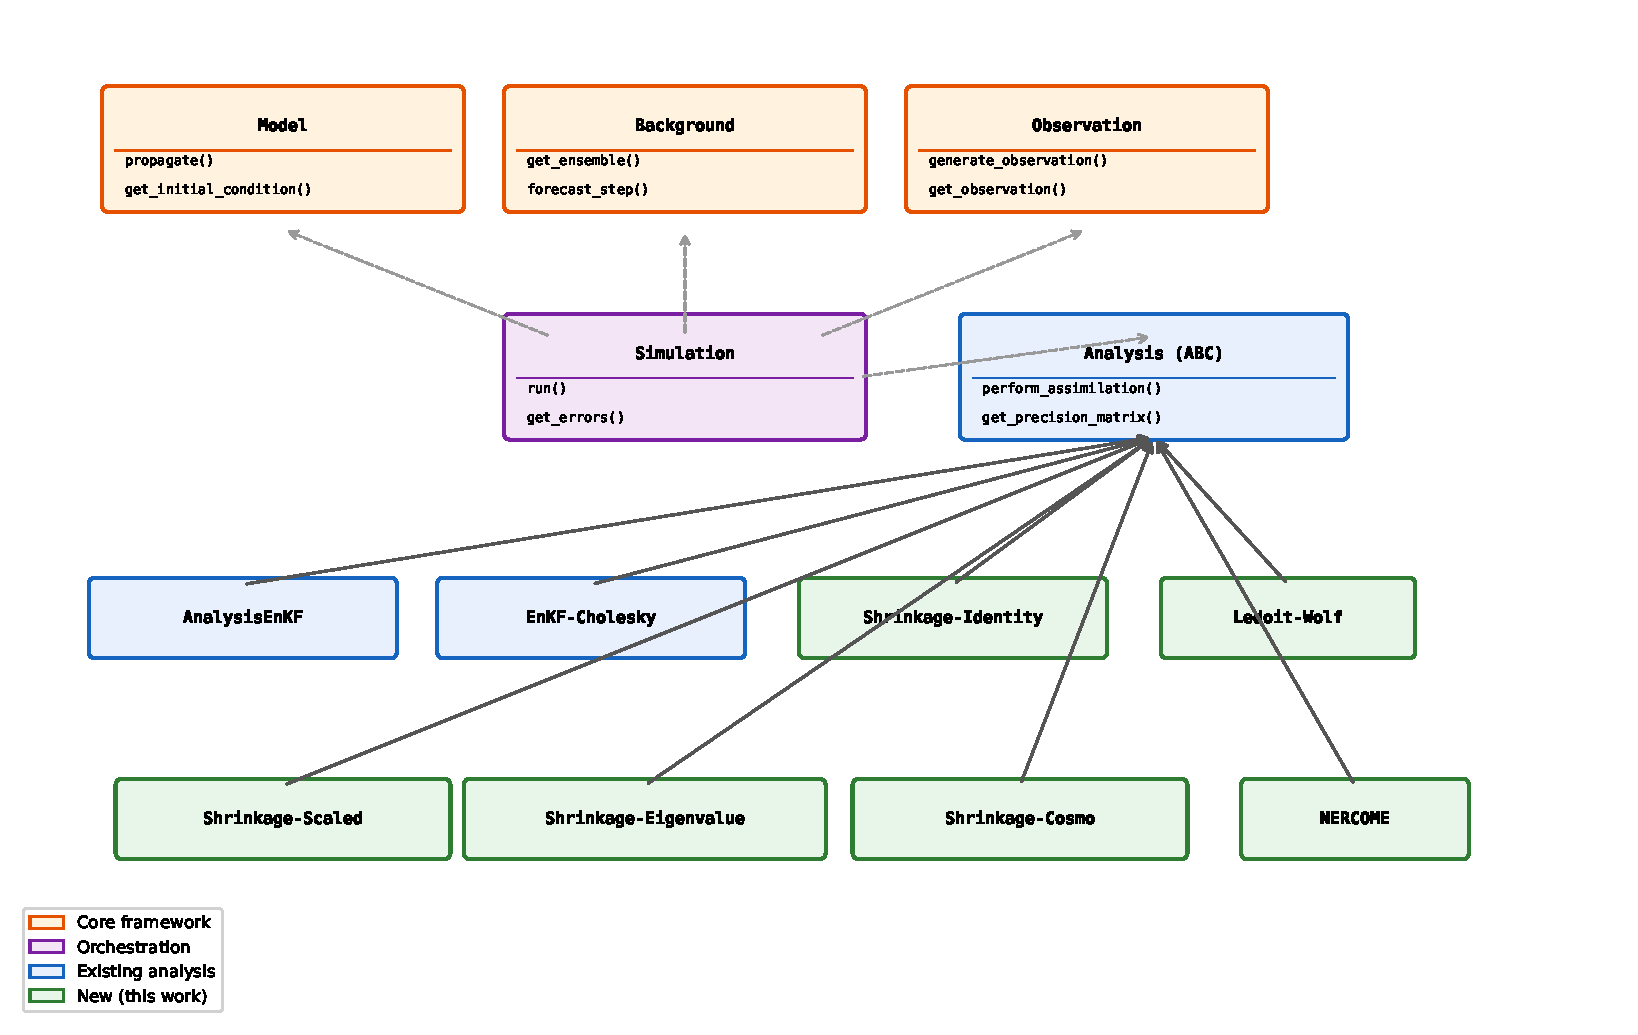
\includegraphics[width=\textwidth]{figures/class_diagram.pdf}
\caption{Class diagram of the TEDA framework, highlighting the new shrinkage estimator classes (shaded). All analysis methods inherit from the abstract \texttt{Analysis} base class and are registered via the \texttt{AnalysisFactory}, enabling interchangeability.}
\label{fig:class_diagram}
\end{figure}

The main classes are \textbf{Model} (abstract base for dynamical systems like Lorenz~96, defining the \texttt{propagate()} interface), \textbf{Background} (manages the ensemble and computes ensemble statistics), \textbf{Observation} (generates synthetic observations and manages $\mathbf{H}$ and $\mathbf{R}$), \textbf{Analysis} (abstract base for assimilation; subclasses override \texttt{perform\_assimilation()}), and \textbf{Simulation} (orchestrates the forecast-analysis cycle and stores results).

New analysis methods are registered via a factory pattern. The \texttt{@register\_analysis} decorator lets users select methods by name at runtime:
\begin{verbatim}
from pyteda.analysis import AnalysisFactory
method = AnalysisFactory.create("EnKF-Shrinkage-Cosmo",
                                 params=config)
\end{verbatim}

\subsection{Shrinkage Estimator Implementations}
\label{sec:estimators}

We implemented four variants of the \emph{direct linear shrinkage estimator for the precision matrix}, three from Looijmans et al.~\cite{looijmans2024comparison} and one novel domain-agnostic adaptation. Each variant corresponds to a different target precision matrix $\boldsymbol{\Pi}_0$. All inherit from the \texttt{Analysis} base class and override \texttt{get\_precision\_matrix()}.

Following Bodnar et al.~\cite{bodnar2016direct} as applied in Looijmans et al.~\cite{looijmans2024comparison}, the direct precision shrinkage estimator combines the raw sample precision $\hat{\boldsymbol{\Pi}}_S = \mathbf{S}^{-1}$ with a structured target~$\boldsymbol{\Pi}_0$:
\begin{equation}
\label{eq:direct_precision}
\boldsymbol{\Pi}_{\text{LS}} = \alpha^* \hat{\boldsymbol{\Pi}}_S + \beta^* \boldsymbol{\Pi}_0,
\end{equation}
where $\alpha^*$ and $\beta^*$ are estimated analytically. The Bodnar formula is derived for the \emph{raw} inverse $\mathbf{S}^{-1}$; the $(1 - n/N_e)$ term in Eq.~\eqref{eq:alpha_star} already accounts for the estimation bias, so applying the Hartlap correction $\gamma = (N_e - n - 2)/(N_e - 1)$~\cite{hartlap2007your} beforehand would alter the formula in a way not derived in the original work.
\begin{align}
\label{eq:alpha_star}
\alpha^* &= 1 - \frac{n}{N_e} - \frac{N_e^{-1} \|\hat{\boldsymbol{\Pi}}_S\|_{\text{tr}}^2 \, \|\boldsymbol{\Pi}_0\|_F^2}{\|\hat{\boldsymbol{\Pi}}_S\|_F^2 \, \|\boldsymbol{\Pi}_0\|_F^2 - \bigl(\text{tr}(\hat{\boldsymbol{\Pi}}_S \boldsymbol{\Pi}_0)\bigr)^2}, \\
\label{eq:beta_star}
\beta^* &= \left(1 - \frac{n}{N_e} - \alpha^*\right) \frac{\text{tr}(\hat{\boldsymbol{\Pi}}_S \boldsymbol{\Pi}_0)}{\|\boldsymbol{\Pi}_0\|_F^2},
\end{align}
where $\|\cdot\|_{\text{tr}}$ is the trace norm and $\|\cdot\|_F$ the Frobenius norm. We clamp both $\alpha^*$ and $\beta^*$ to $[0,1]$ with $\alpha^* + \beta^* \leq 1$ as a finite-sample safeguard; Bodnar et al.\ show these constraints hold asymptotically.

The four variants differ only in their choice of~$\boldsymbol{\Pi}_0$.

\subsubsection{Identity Target.}

The simplest target: $\boldsymbol{\Pi}_0 = \mathbf{I}_n$, assuming independent unit-variance priors. Implemented as \texttt{Analysis\-EnKF\-Direct\-Precision\-Shrinkage\-Identity}.

\begin{algorithm}[t]
\caption{Direct Precision Shrinkage (Identity Target)}
\label{alg:identity}
\begin{algorithmic}[1]
\REQUIRE Deviation matrix $\mathbf{DX} \in \mathbb{R}^{n \times N_e}$
\STATE Compute sample covariance: $\mathbf{S} = \frac{1}{N_e-1} \mathbf{DX} \, \mathbf{DX}^T$
\STATE Compute sample precision: $\hat{\boldsymbol{\Pi}}_S = \mathbf{S}^{-1}$
\STATE Set target: $\boldsymbol{\Pi}_0 = \mathbf{I}_n$
\STATE Compute $\alpha^*, \beta^*$ via Eqs.~\eqref{eq:alpha_star}--\eqref{eq:beta_star}
\RETURN $\boldsymbol{\Pi}_{\text{LS}} = \alpha^* \hat{\boldsymbol{\Pi}}_S + \beta^* \boldsymbol{\Pi}_0$
\end{algorithmic}
\end{algorithm}

The identity target carries no domain-specific information, but the direct precision formulation still guarantees a valid precision matrix---unlike inverting a shrunk covariance, which can amplify estimation error.

\subsubsection{Eigenvalue Target.}

Uses the eigenvalue-based target from Looijmans et al.\ Eq.~(15): a diagonal matrix of the sorted eigenvalues of $\hat{\boldsymbol{\Pi}}_S$. TEDA class: \texttt{Analysis\-EnKF\-Direct\-Precision\-Shrinkage\-Eigenvalues}.

\begin{algorithm}[t]
\caption{Direct Precision Shrinkage (Eigenvalue Target)}
\label{alg:eigenvalue}
\begin{algorithmic}[1]
\REQUIRE Deviation matrix $\mathbf{DX} \in \mathbb{R}^{n \times N_e}$
\STATE Compute $\mathbf{S}$, $\hat{\boldsymbol{\Pi}}_S$ as in Algorithm~\ref{alg:identity} (Steps 1--2)
\STATE Compute eigenvalues $e_1 \leq \cdots \leq e_n$ of $\hat{\boldsymbol{\Pi}}_S$
\STATE Set target: $\boldsymbol{\Pi}_0^{(1)} = \text{diag}(e_1, \ldots, e_n)$
\STATE Compute $\alpha^*, \beta^*$ via Eqs.~\eqref{eq:alpha_star}--\eqref{eq:beta_star}
\RETURN $\boldsymbol{\Pi}_{\text{LS}} = \alpha^* \hat{\boldsymbol{\Pi}}_S + \beta^* \boldsymbol{\Pi}_0^{(1)}$
\end{algorithmic}
\end{algorithm}

This target retains the spectral information of the sample precision while zeroing out off-diagonal correlations. It requires no external domain knowledge. This is the first precision matrix target ($\boldsymbol{\Pi}_0^{(1)}$) evaluated in Looijmans et al.~\cite{looijmans2024comparison}.

\subsubsection{Scaled Identity Target (novel adaptation).}

We propose this variant to apply the Bodnar framework without domain-specific priors. Since power spectrum data $C_\ell$ and mode counts $N_\ell$ are unavailable outside cosmology, we use empirical per-variable variances: $\boldsymbol{\Pi}_0 = \text{diag}(1/(2\sigma_1^2), \ldots, 1/(2\sigma_n^2))$, where $\sigma_i^2$ are the diagonal entries of $\mathbf{S}$. The factor of~2 mirrors the $2/N_\ell$ scaling of the cosmological target. This is \emph{not} from Looijmans et al.; its experimental results (Section~\ref{sec:results}) illustrate how much direct precision shrinkage performance depends on domain-specific target knowledge. TEDA class: \texttt{Analysis\-EnKF\-Direct\-Precision\-Shrinkage\-Identity\-Scaled}.

\subsubsection{Cosmological Target.}

This variant implements the analytical cosmological target from Looijmans et al.\ Eqs.~(14) and (16), available as \texttt{Analysis\-EnKF\-Direct\-Precision\-Shrinkage\-Cosmo}. The target precision is the inverse of the theoretical Gaussian power spectrum covariance:

\begin{algorithm}[t]
\caption{Direct Precision Shrinkage (Cosmological Target)}
\label{alg:cosmo}
\begin{algorithmic}[1]
\REQUIRE Deviation matrix $\mathbf{DX}$, power spectrum $C_\ell$, mode counts $N_\ell$
\STATE Compute $\mathbf{S}$, $\hat{\boldsymbol{\Pi}}_S$ as in Algorithm~\ref{alg:identity} (Steps 1--2)
\FOR{each data element $i$ mapped to multipole $\ell_i$}
    \STATE Compute diagonal covariance target: $T^{(2)}_{ii} = \frac{2}{N_{\ell_i}} C_{\ell_i}^2$
\ENDFOR
\STATE Set target precision: $\boldsymbol{\Pi}_0^{(2)} = (\mathbf{T}^{(2)})^{-1}$
\STATE Compute $\alpha^*, \beta^*$ via Eqs.~\eqref{eq:alpha_star}--\eqref{eq:beta_star}
\RETURN $\boldsymbol{\Pi}_{\text{LS}} = \alpha^* \hat{\boldsymbol{\Pi}}_S + \beta^* \boldsymbol{\Pi}_0^{(2)}$
\end{algorithmic}
\end{algorithm}

Here $T^{(2)}_{ii} = (2/N_{\ell_i}) C_{\ell_i}^2$ encodes the Gaussian cosmic variance at multipole~$\ell_i$~\cite{hamilton2006measuring}. When the assumed power spectrum model is close to the truth, this target provides a stronger shrinkage direction than the identity or eigenvalue alternatives.

\subsection{Integration and Usage}
\label{sec:integration}

All estimator classes are registered in the analysis factory and follow TEDA's modular design: each method lives in its own file under \texttt{pyteda/analysis/}, new variants can be added by subclassing \texttt{Analysis} and applying \texttt{@register\_analysis}, and all classes share the same interface so they can be compared in a single simulation run. The code includes docstrings with mathematical notation matching this paper, and default parameters are set to produce reasonable results without manual tuning.

A typical comparative experiment requires only changing the method name:
\begin{verbatim}
methods = ["EnKF", "EnKF-Cholesky",
           "EnKF-Shrinkage-Identity",
           "EnKF-Shrinkage-Cosmo",
           "EnKF-Shrinkage-Eigenvalues"]
for name in methods:
    sim = Simulation(model, background,
                     AnalysisFactory.create(name),
                     observation)
    sim.run()
\end{verbatim}
